\subsection{Domino Tiling}
We will consider the problem of tiling a square grid with dominos.
This problem has a long histor and various importtant applications in statistical physics.
Specifically, we will focus on the local generation of domino tilings from the uniform distribution.

\subsection{$2\times n$ Domino Tiling}
The simplest version of the problem is one where we are given a $2\times n$ grid (Figure~\ref{fig:dom2}.
The queries will be as an index, and the generator should report the orientation of the domino at the $i^{th}$ position in the grid.
\begin{figure}[htbp]
    \centering
    %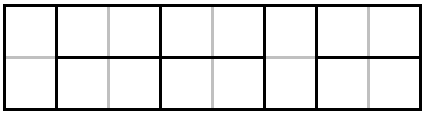
\includegraphics[width=\textwidth]{images/domino2}
    \caption{}
    \label{fig:dom2}
\end{figure}

It is a well known result \todo{cite} that the number of tilings of a $2\times n$ grid is exactly $F_n$.

To aid with generalization, we will instead allow the generator to respond with the splitting boundary of the current tiling instead.
For example, in Figure~\ref{fig:b20}, the boundary is a vertical line at the specified position.
In Figure~\ref{fig:b21}, the boundary is horizontal, indicating that there are two horizontal dominos at that location.
Note that Figure~\ref{fig:b22} is impossible for a $2\times n$ grid.
It should be clear that this query model is equivalent.

\begin{figure}[h]
    \centering
    \subfloat[][]{
        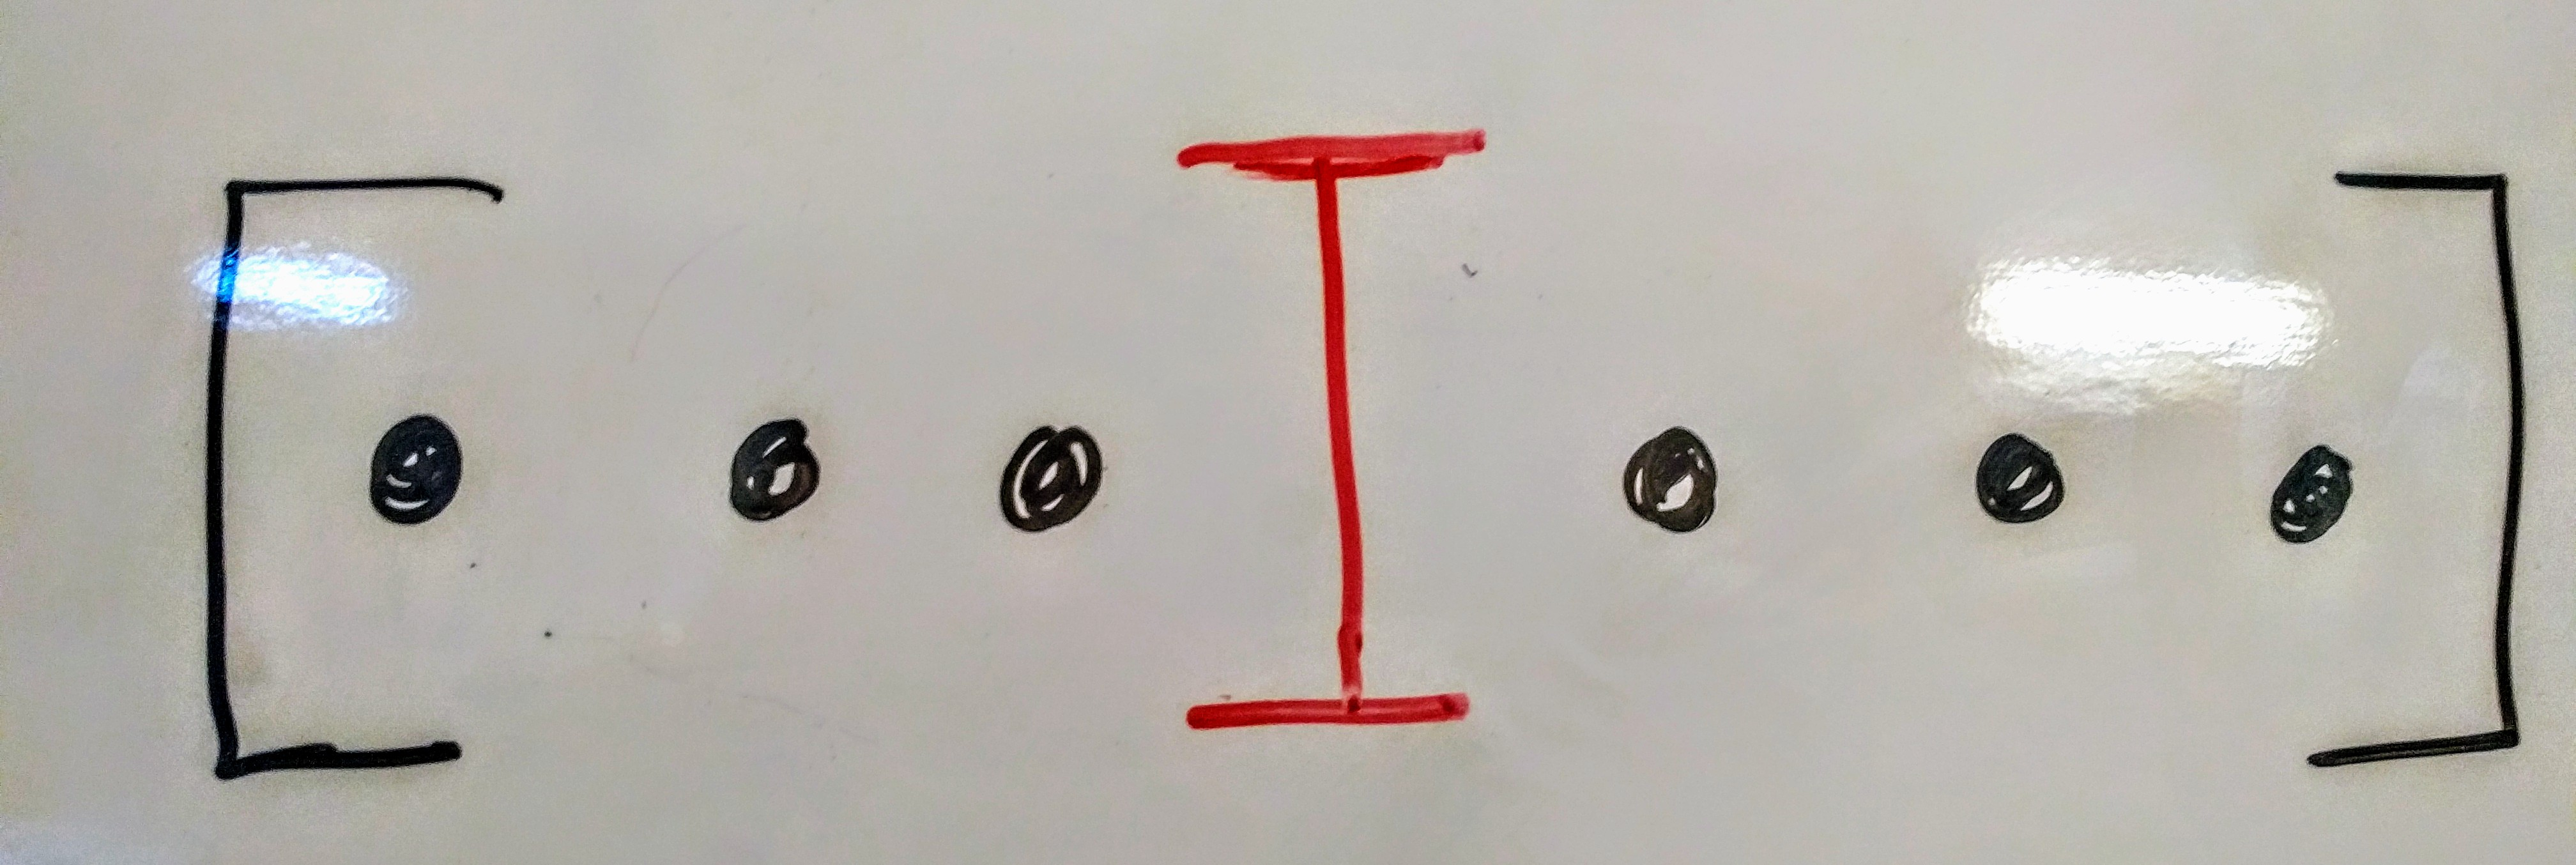
\includegraphics[width=0.5\linewidth]{images/tile2-0.jpg}
        \label{fig:b20}
    }
    \subfloat[][]{
        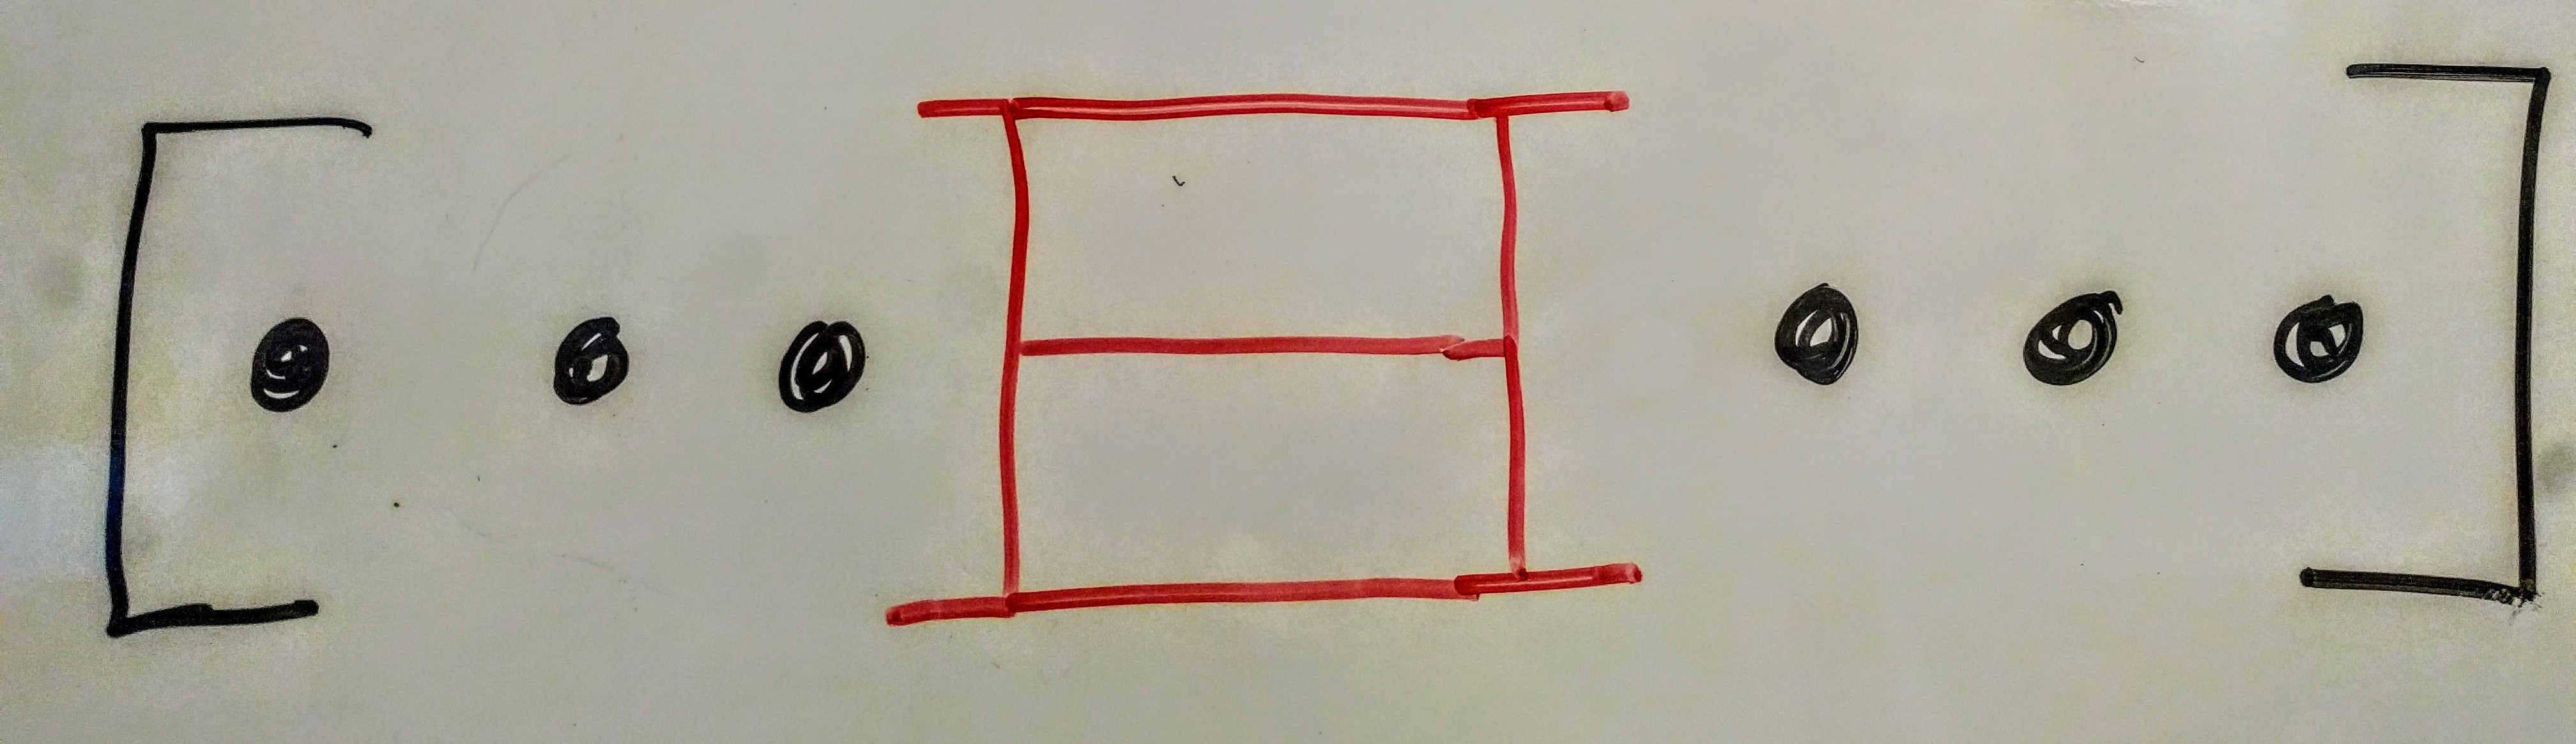
\includegraphics[width=0.5\linewidth]{images/tile2-1.jpg}
        \label{fig:b21}
    }
    \subfloat[][]{
        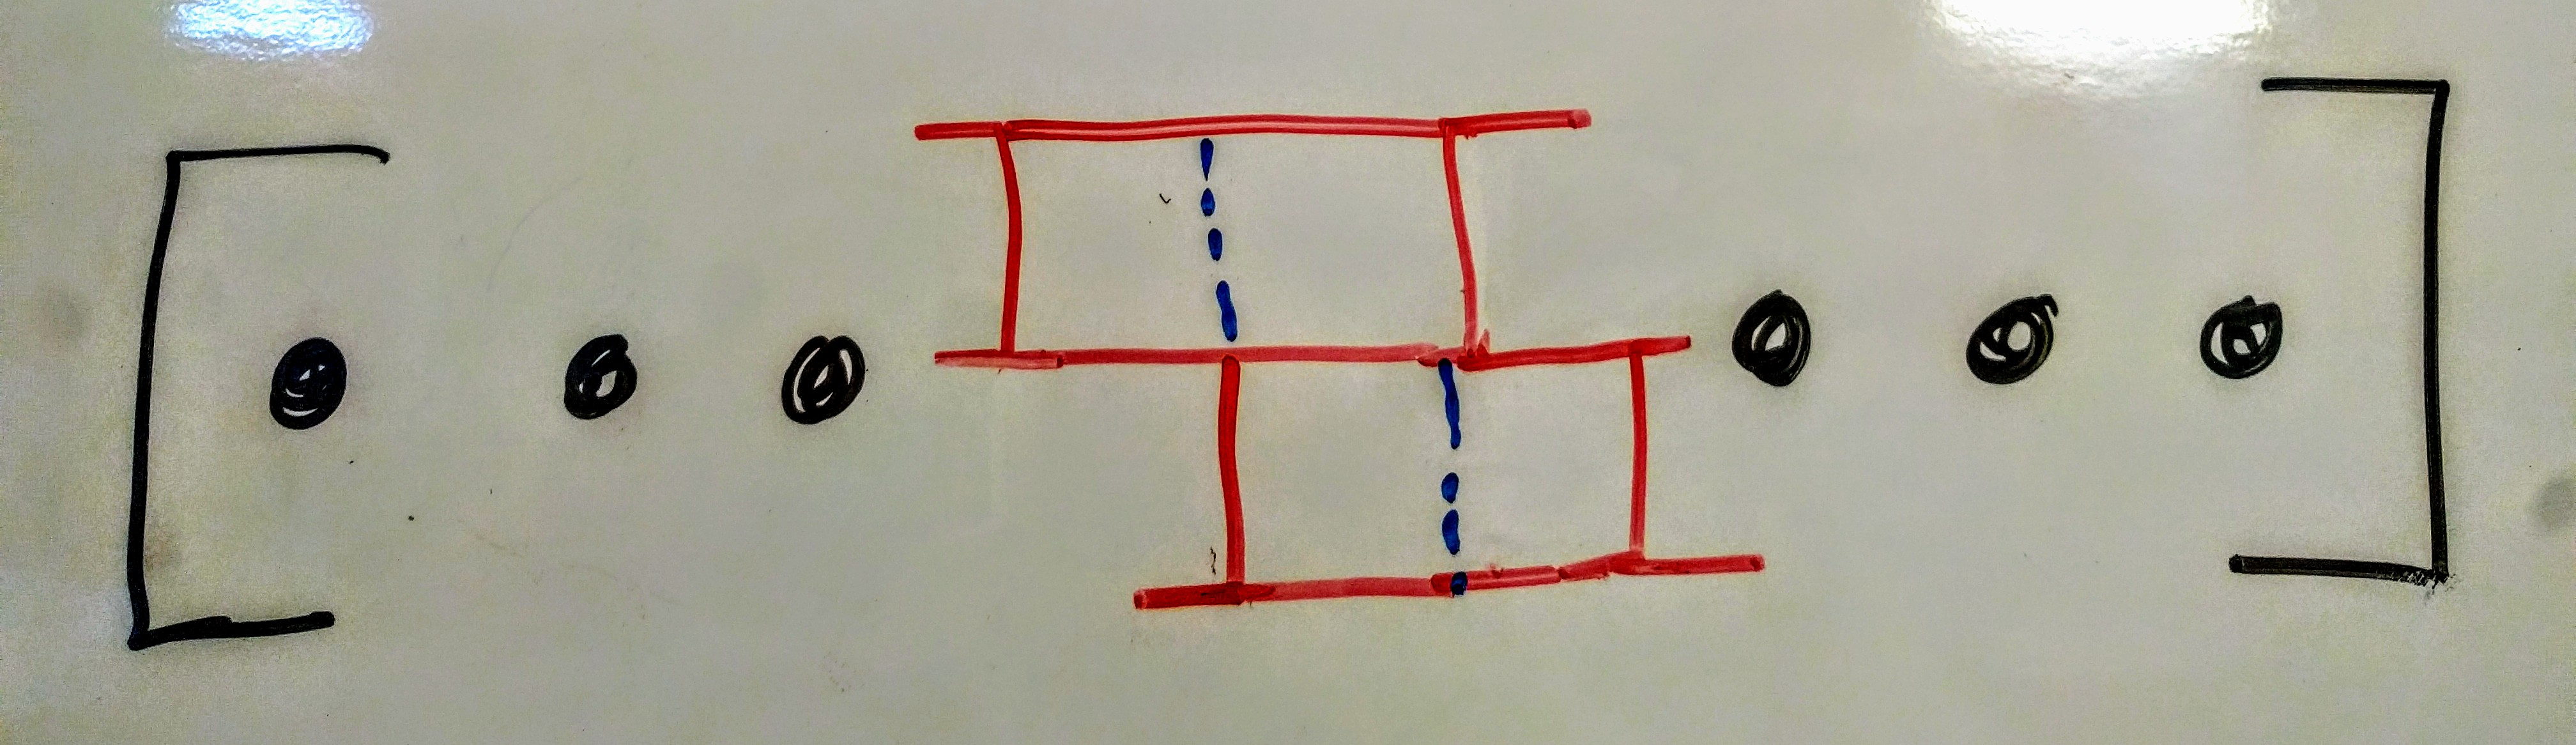
\includegraphics[width=0.5\linewidth]{images/tile2-2.jpg}
        \label{fig:b22}
    }
    \caption{Caption for this figure with two images}
    \label{fig:boundary2}
\end{figure}

Now, consider a query to the location $i$, such that all positions between $i-a$ and $i+b$ have not been queriesd so far.
So, there is a blank $2\times(a+b)$ size sub-grid that we have to sample from.
Let us consider the number of possible tilings resulting from each possible splitting boundary.
\begin{enumerate}
    \item Vertical Boundary -- This indicates that we divide the region into two sub-grids with sizes
          $2\times a$ and $2\times b$.
          So, the total number of possible tilings is exactly $F_a\cdot F_b$.
    \item Horizontal Boundary -- This indicates that we divide the region into two sub-grids with sizes
          $2\times (a-1)$ and $2\times (b-1)$.
          So, the total number of possible tilings is exactly $F_{a-1}\cdot F_{b-1}$.
\end{enumerate}

So the probabilities are computed as $\frac{F_a\cdot F_b}{F_a\cdot F_b + F_{a-1}\cdot F_{b-1}}$
and $\frac{F_{a-1}\cdot F_{b-1}}{F_a\cdot F_b + F_{a-1}\cdot F_{b-1}}$.
Now, we face the issue of approximating these fractions.
If either of the values $a$ or $b$ are less than $\Theta(\sqrt n)$,
then we can compute the exact value of the corresponding $F_a$ or $F_b$.
Otherwise, we use Lemma~\ref{lem:rat_conv} to approximate $F_a=\phi\cdot F_{a-1}$ and $F_b=\phi\cdot F_{b-1}$.
So, the probability of the vertical boundary becomes
$$
\frac{F_a\cdot F_b}{F_a\cdot F_b + F_{a-1}\cdot F_{b-1}} = \frac{\phi^2}{\phi^2+1}
$$
Similarly, the probability of a horizontal split with a top and bottom domino becomes $1/(\phi^2+1)$.
Note that this also determines the two adjacent boundaries.

The only information we needed to make this query was the extent of the un-queried interval $[i-a, i+b]$.
We can use any standard data-structure that allows insertion in positions $\{1, 2\cdots,n+1\}$,
and provides successor and predecessor queries.

Here's we can be fancy and use Van-Emde-Boas trees to get a $\Bo(\log\log n)$ query time.
However, in some cases, the exact value of a Fibonacci number still needs to be computed, and this takes $\Bo(\log n)$ time.
The faster queries only work when the new query is "far enough" ($\Bo(\log n)$ distance) away from all previous queries.

